\documentclass[a4paper,12pt]{article}
\usepackage[pdftex]{graphicx}

\begin{document}

\title{Architectural Patterns and Styles - Notes}
\author{Priscilla Madigoe}
\date{08 March 2016}
\maketitle
 
\section{Architectural Patterns}

\subsection{Introduction}
Often times source code needs to be organised so that clear roles, responsibilities and relationships of different modules of the code can be well defined. Architectural patterns help in making this possible and numerous types will be discussed in this section. Using these patterns, code becomes easier to maintain, manage and visualise. They also make understanding of how each component works in a system easier. They are reusable solutions to a commonly occuring problem in Software Architecture within a given context.

\subsection{Types of Architectural Patterns}

\begin{itemize}
\item Layers Pattern
\item Client-server
\item Representational State Transfer (REST)
\item Master-slave
\item Pipe-filter
\item Broker Pattern
\item Peer-to-peer
\item Event-bus Pattern
\item Model View Controller
\item Blackboard Pattern
\item Interpreter
\end{itemize}

\subsection{Architectural Patterns Proposed for PAPERS}

\subsubsection{Model View Controller}
\begin{itemize}
\item{Background}
\newline
\newline
In the Model-View-Controller Pattern, an interactive application is divided into three parts: the Model is an object representing the data and activities, the View displays information to the user and the Controller offers a way to change the state of the Model.

\begin{figure}[H]				
	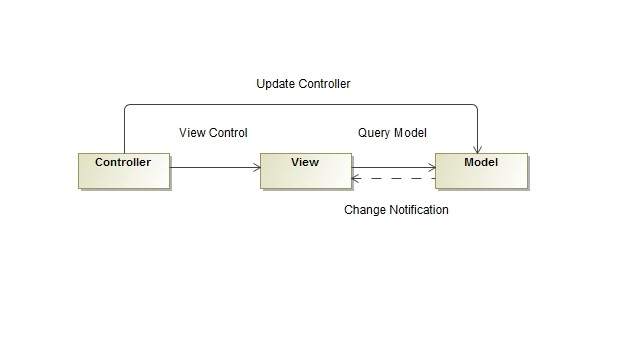
\includegraphics[width=4in]{../Diagrams/Architectural Patterns/Model View Controller.jpg}
	\caption{ Model View Controller }
\end{figure}

\end{itemize}


\end{document}